\documentclass{article}

% Language setting
% Replace `english' with e.g. `spanish' to change the document language
\usepackage[english]{babel}

% Set page size and margins
% Replace `letterpaper' with `a4paper' for UK/EU standard size
\usepackage[letterpaper,top=2cm,bottom=2cm,left=3cm,right=3cm,marginparwidth=1.75cm]{geometry}

% Useful packages
\usepackage{amsmath}
\usepackage{graphicx}
\usepackage[colorlinks=true, allcolors=blue]{hyperref}
\usepackage{float}

\title{Program Assignment 1}
\author{Zhangyuan Wang}

\begin{document}
\maketitle


%\begin{abstract}
%Your abstract.
%\end{abstract}


\section{K-means}
Kmeans algorithm is an iterative algorithm used to cluster the given set of data into different groups by randomly choosing the data points as Centroids C1, C2, and so on and then calculating the distance between each data point in the data set to the centroids and based on the distance, all the data points closer to each centroid is labeled with 0, 1 and so on and then the average of all the data points labeled with 0, 1 and so on is calculated separately and made as the new centroid C1, C2 and so on and the same process is repeated until the centroids are converged to a fixed point.I tried different K from 1 to 10. The best result is K=4 as illustrated  in Fig \ref{fig:kmeans} .\par
\begin{figure} [H]
\centering
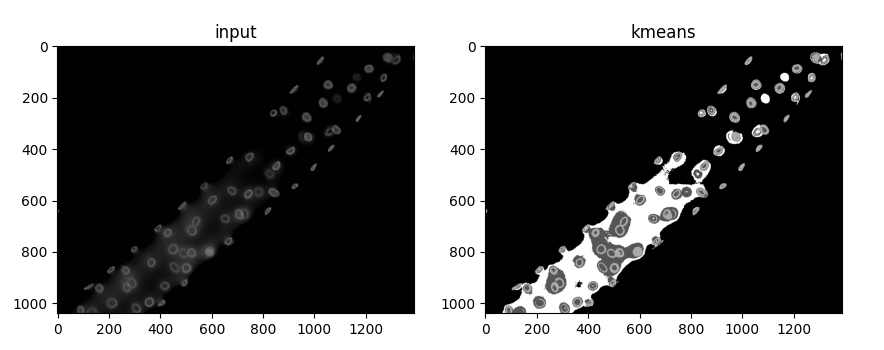
\includegraphics[width=0.6\textwidth]{Figure_1.png}
\caption{\label{fig:kmeans}K-means operation.}
\end{figure}
\subsection{Morphological Operations}
I separate the four different labels with background filled into a binary image. The third label of figure is all the cells as in Fig \ref{fig:3means} . But it is hard to count the number of the cells as some cells are overlapping with each other and so much noise in it. Therefore, I choose to operate it with erosion. Additionally, combine it with the original figure, we can see the contours. The result is shown in Fig \ref{fig:erosion}.
\begin{figure} [H]
\centering
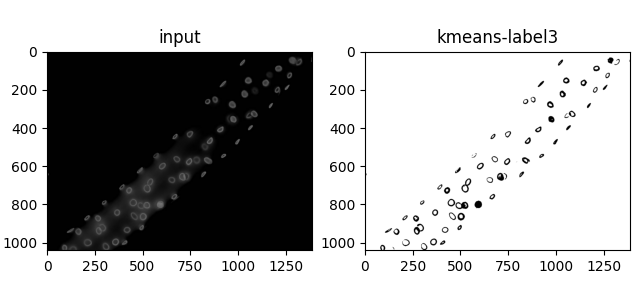
\includegraphics[width=0.6\textwidth]{Figure_2.png}
\caption{\label{fig:3means}The third label of figure.}
\end{figure}

\begin{figure} [H]
\centering
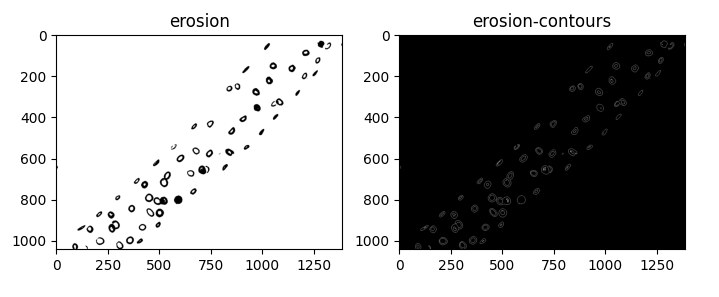
\includegraphics[width=0.6\textwidth]{Figure_3.png}
\caption{\label{fig:erosion}Erosion operation.}
\end{figure}

I use the function \emph{cv2.drawContours} to find the outer contours in Fig \ref{fig:Countours}. The number of the contours is equal to the number of the cells as in Fig \ref{fig:number}.
\begin{figure} [H]
\centering
\includegraphics[width=0.6\textwidth]{TheContours.jpg}
\caption{\label{fig:Countours}The outer contours.}
\end{figure}

\begin{figure} [H]
\centering
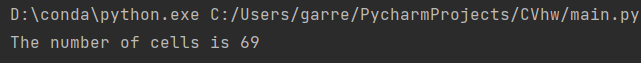
\includegraphics[width=0.6\textwidth]{number.png}
\caption{\label{fig:number}The number of the cells.}
\end{figure}

\section{Mean-shift}
Meanshift is a very useful method to keep track of a particular object inside a video. Meanshift can separate the static background of a video and the moving foreground object.

The idea behind meanshift is that in meanshift algorithm every instance of the video is checked in the form of pixel distribution in that frame. We define an initial window, generally a square or a circle for which the positions are specified by ourself which identifies the area of maximum pixel distribution and tries to keep track of that area in the video so that when the video is running our tracking window also moves towards the region of maximum pixel distribution. The direction of movement depends upon the difference between the center of our tracking window and the centroid of all the k-pixels inside that window.

Similarly, using the python package \emph{sklearn.cluster} we can define the bandwidth and run mean-shift algorithm conveniently. The mean-shift algorithm is more completed than k-means so that it takes more time. I diliver it to the baidu Aistudio. The result is shown in Fig \ref{fig:MsFigure_1}.
\begin{figure} [H]
\centering
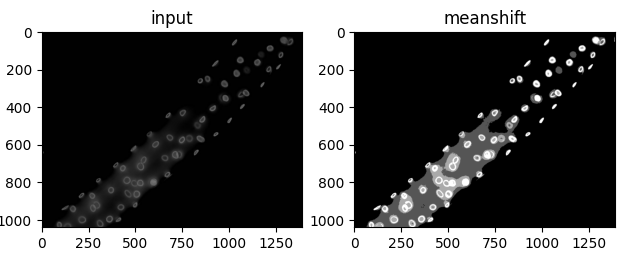
\includegraphics[width=0.6\textwidth]{MsFigure_1.png}
\caption{\label{fig:MsFigure_1}Mean-shift.}
\end{figure}
The result shows that the unsupervised algorithm divided the Figure into 4 labels. The 4 labels are also shown in Fig \ref{fig:MsFigure_2}.
\begin{figure} [H]
\centering
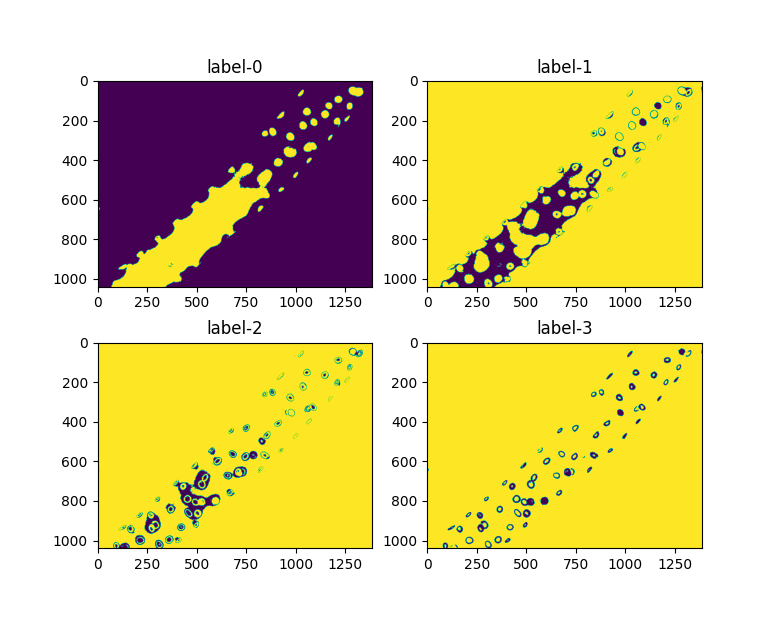
\includegraphics[width=0.6\textwidth]{MsFigure_2.png}
\caption{\label{fig:MsFigure_2}The four labels of Mean-shift.}
\end{figure}
Also, use erosion and erosion-contours operation is shown in Fig \ref{fig:MsFigure_3}.
\begin{figure} [H]
\centering
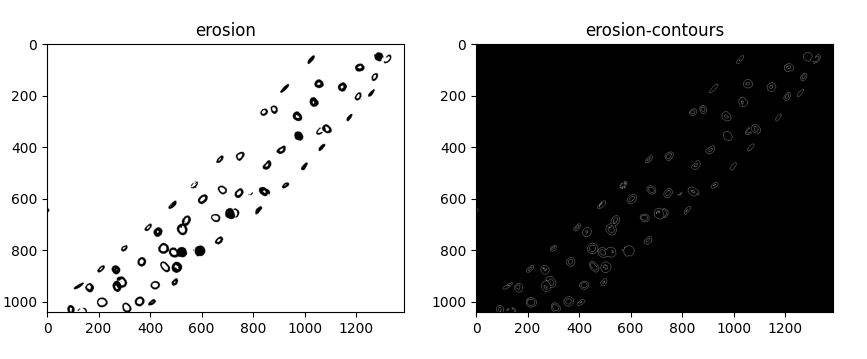
\includegraphics[width=0.6\textwidth]{MsFigure_3.png}
\caption{\label{fig:MsFigure_3}Erosion operation.}
\end{figure}
The contours and the number of which is shown in Fig \ref{fig:Countours2} and Fig \ref{fig:number2}. From the result, the mean-shift  algorithm is more accurate than the K-means.
\begin{figure} [H]
\centering
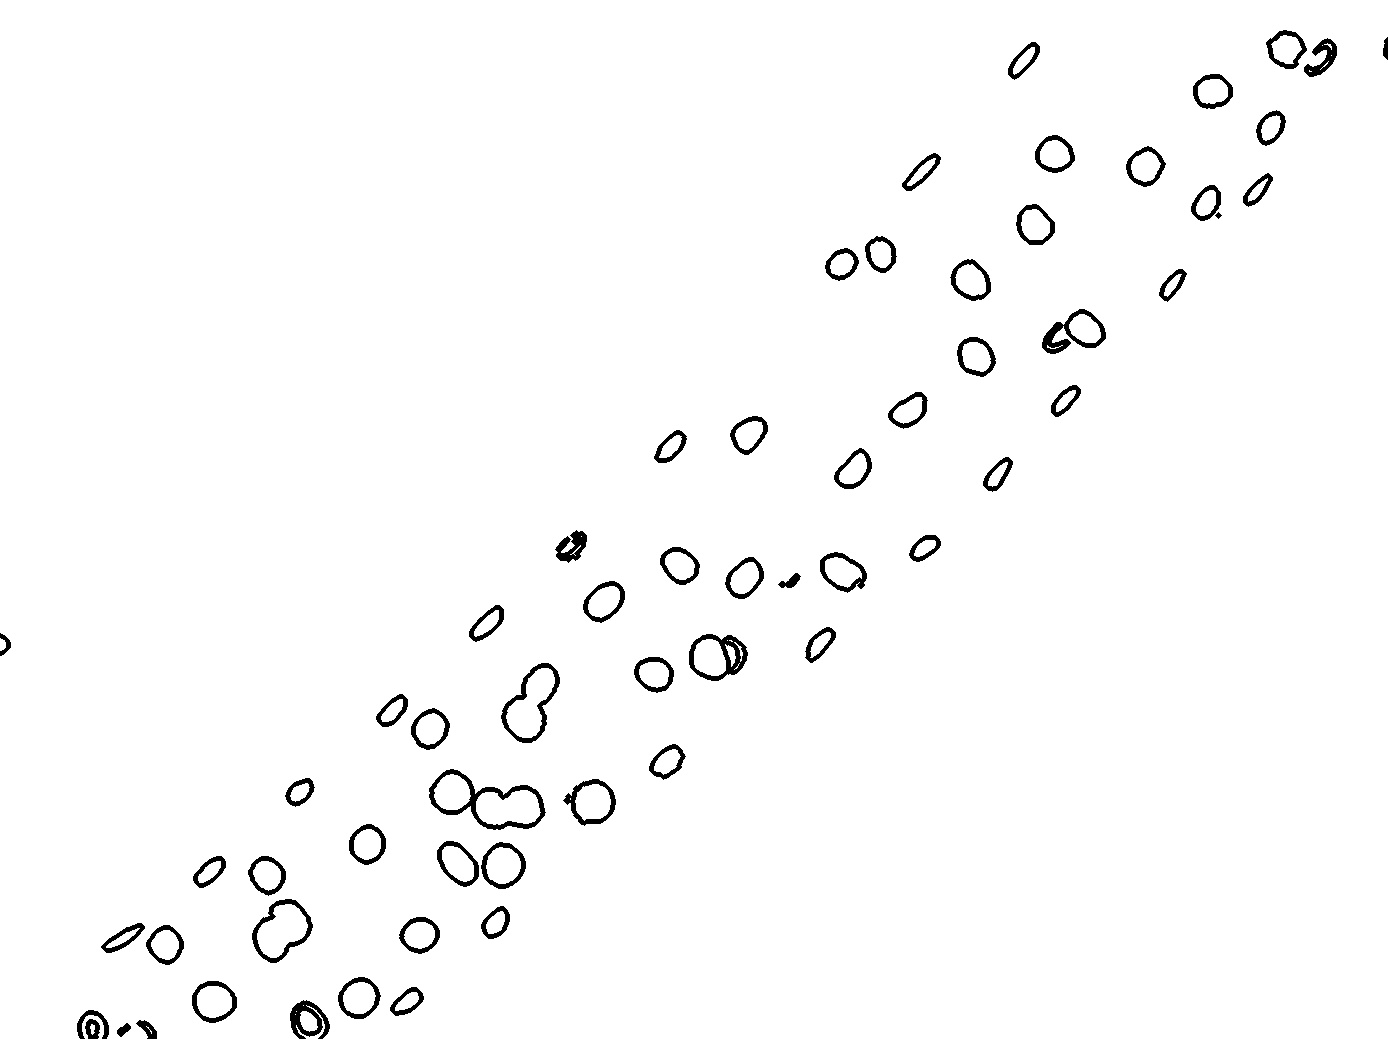
\includegraphics[width=0.6\textwidth]{TheContours2.jpg}
\caption{\label{fig:Countours2}The outer contours.}
\end{figure}

\begin{figure} [H]
\centering
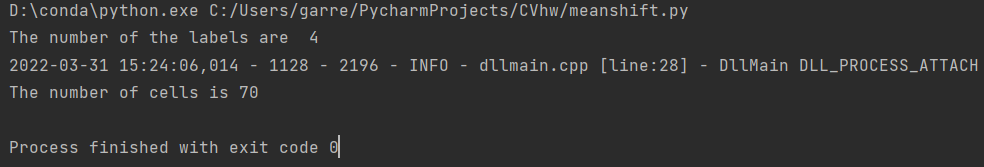
\includegraphics[width=0.6\textwidth]{number2.png}
\caption{\label{fig:number2}The number of the cells.}
\end{figure}
\section{Active Contour}
The active contour model is a method to fit open or closed splines to lines or edges in an image 1. It works by minimising an energy that is in part defined by the image and part by the spline’s shape: length and smoothness. The minimization is done implicitly in the shape energy and explicitly in the image energy.

In the following example the active contour model is used to segment one cell from the rest of an image by fitting a closed curve to the edges of the cell and  typically it is a good idea to smooth images a bit before analyzing, as done in the Fig \ref{fig:AC}.

We initialize a circle around the astronaut’s face and use the default boundary condition\\ \emph{boundary\_condition='periodic'}  to fit a closed curve. The default parameters \emph{w\_line=0}, \emph{w\_edge=1} will make the curve search towards edges, such as the boundaries of the face.
\begin{figure} [H]
\centering
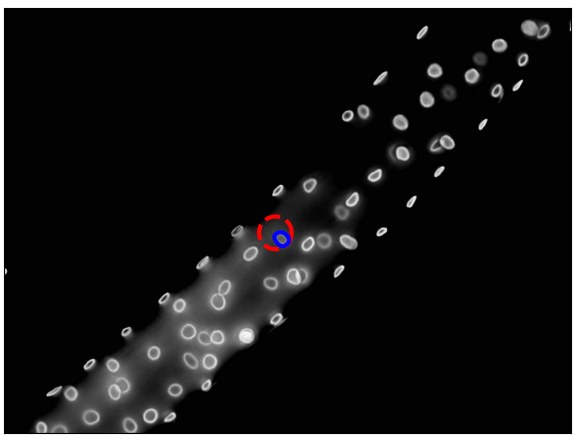
\includegraphics[width=0.6\textwidth]{AC.png}
\caption{\label{fig:AC}Active contour.}
\end{figure}

\end{document}
